\documentclass[uplatex,a4paper,12pt]{jsarticle}
% \documentclass[uplatex,a4paper,12pt,draft]{jsarticle}

%% フォント
%\usepackage{newtxtext,newtxmath}
%% 図、文字色
\usepackage[dvipdfmx]{graphicx,xcolor}
%% ハイパーリンク
\usepackage[dvipdfmx]{hyperref}
%% しおりの日本語
\usepackage{pxjahyper}
%% しおりに節番号を含める、リンクの枠を出力しない
\hypersetup{
  bookmarksnumbered=true,
  hidelinks=true,
  colorlinks=false,
}
%% 特殊記号
\usepackage{textcomp}
%% URL
\usepackage{url}
%% 表
%\usepackage{multirow}
%% 参照漏れチェック
%\usepackage{refcheck}

\usepackage{subcaption}

% 図と表の表記
\renewcommand{\figurename}{Fig.}
\renewcommand{\tablename}{Table.}
\newcommand{\figref}[1]{\figurename~\ref{#1}}
\newcommand{\tabref}[1]{\tablename~\ref{#1}}

\usepackage[top=30truemm,bottom=30truemm,left=30truemm,right=30truemm]{geometry}

\begin{document}

% 表紙
\begin{picture}(420,520)(-20,20)
%契約番号(必須)
\put(330,470){\makebox(50,5)[l]{\normalsize{2023情財第 XXX 号}}} %「XXX」はプロジェクトごとの番号に置き換える
%事業名(必須)
\put(140,350){\makebox(100,15)[c]{\LARGE{2023年度未踏IT人材発掘・育成事業}}}
%プロジェクト名
\put(140,320){\makebox(100,15)[c]{\LARGE{ぬいぐるみ専用の組み込みAIモジュールの開発}}}
% \put(140,290){\makebox(100,15)[c]{\LARGE{契約名2行目(必要なら)}}}
\put(140,290){\makebox(100,15)[c]{\LARGE{成果報告書}}} %2行目がなければ\put(140,290)
%クリエータ名1(必須、人数に応じて\putの位置を調整)
\put(140,140){\makebox(100,10)[c]{\Large{クリエータ:小山 高}}}
%クリエータ名2(必須、人数に応じて\putの位置を調整)
% \put(140,110){\makebox(100,10)[c]{\Large{      姓 名}}}
% 担当PM名(クリエータ2がいなければ\put(140,100)
\put(140,100){\makebox(100,10)[c]{\Large{担当PM:稲見 昌彦}}}
%日付(必須、通常は契約最終日、クリエータ2がいなければ\put(140,60)
\put(140,60){\makebox(100,15)[c]{\Large{2024年3月8日}}}
\end{picture}
\thispagestyle{empty}
\clearpage

\tableofcontents
\thispagestyle{empty}
\clearpage

% 本文
\pagenumbering{arabic}
\setcounter{page}{1}

\section{要約}
本プロジェクトでは、様々な種類のぬいぐるみをロボット化するための、ぬいぐるみ専用の組み込みAIモジュールを提案・実装した。
ぬいぐるみロボットでは、人の好みに寄り添うために、多くの種類のぬいぐるみに対応する必要がある。
そこで、ぬいぐるみロボットを、機械的・電気的要素を含む共通の骨格とぬいぐるみを成す毛皮、ソフトウェアによる知能という三要素に分割して解決したのが本プロジェクトの特徴である。
本プロジェクトでは実際にぬいぐるみロボットを製作し、共通の内部骨格を用いたぬいぐるみ部分の換装の検証や、人とのインタラクションの検証を行った。

\section{背景及び目的}
本プロジェクトでは、現代を生きる若者の孤独に着目し、彼らの生活様式に即した癒やしの手段としてぬいぐるみロボットを提案する。


\subsection{ペットによる癒やし}
2020年に始まった新型コロナウイルスの流行によって大学ではオンライン授業が行われ、同時に学生同士のつながりが希薄になった。

そこで、コロナ禍の癒やしや巣ごもり需要として、ペットの飼育がブームとなった。

しかし、一人暮らしの大学生がペットを飼うことは容易ではない。


\subsection{愛玩用ロボット}
ペットと似て、愛玩用ロボットも多数存在する。

例えば、犬のような外見をした家庭用ロボットaibo~\cite{web_aibo}、アザラシのような介護現場でも用いられるロボットのパロ~\cite{web_paro}、車輪で駆動する家庭用ロボットLOVOT~\cite{web_lovot}などが存在する(\figref{fig:previous_robots_expensive})。
これらはセンサを多用することでユーザの振る舞いに呼応する機能が埋め込まれており、30万円~50万円で販売されている。

一方で、手のひらサイズのロボットMoflin~\cite{web_moflin}や可動式の尻尾付きのQoobo~\cite{web_qoobo}、ぬいぐるみに縫い付けて使用するボタン型スピーカーpechat~\cite{web_pechat}(※2024年2月で販売終了)といった5万円以下の比較的安価な愛玩用ロボットも存在する(\figref{fig:previous_robots_inexpensive})。
これらは機能や用途を限定しつつもユーザに安らぎや楽しみをもたらすことを目指している。

しかし、これらロボットはまだ市場に出回っておらず、人々認知度も低い。
さらに、工業製品であるがゆえに同型のロボットは多少の色違いこそあれ、基本的にはすべて同じ形である。
これでは、愛玩の対象として重要な、自分の目の前の相手がこの世にただ一人しかいないことから来る愛着、つまりオンリーワンの要素に乏しい。


\begin{figure}[htbp]
  \centering
  \begin{minipage}[c]{0.32\linewidth}
    \centering
    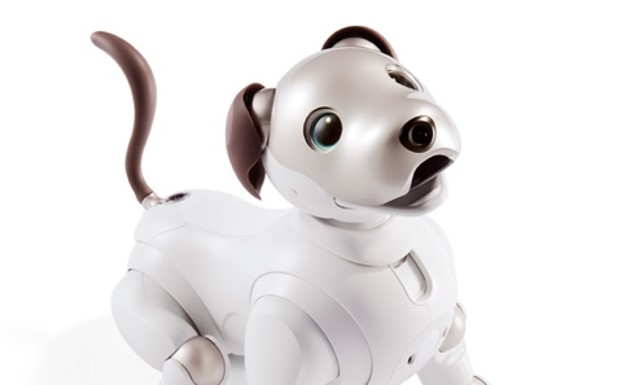
\includegraphics[keepaspectratio,width=4cm,clip]{images/previous_robots/aibo.jpg}
    \subcaption{aibo~\cite{web_aibo}}
    \label{fig:aibo}
  \end{minipage}
  \begin{minipage}[c]{0.32\linewidth}
    \centering
    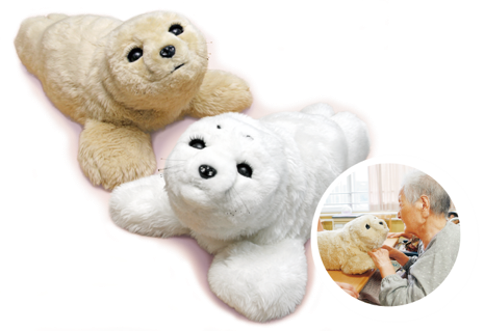
\includegraphics[keepaspectratio,width=4cm,clip]{images/previous_robots/paro.png}
    \subcaption{パロ~\cite{web_paro}}
    \label{fig:paro}
  \end{minipage}
  \begin{minipage}[c]{0.32\linewidth}
    \centering
    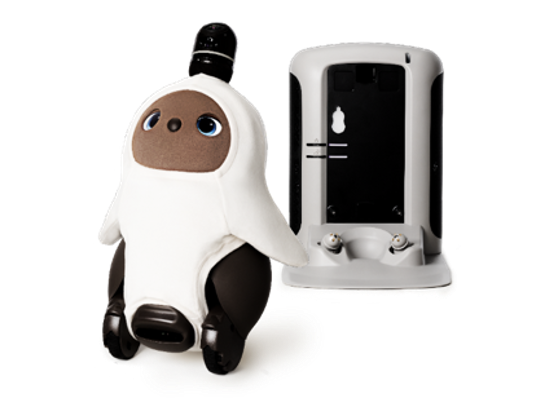
\includegraphics[keepaspectratio,width=4cm,clip]{images/previous_robots/lovot.png}
    \subcaption{LOVOT~\cite{web_lovot}}
    \label{fig:lovot}
  \end{minipage}
  \caption{愛玩用ロボットの例(高価格帯)}
  \label{fig:previous_robots_expensive}
\end{figure}

\begin{figure}[htbp]
  \centering
  \begin{minipage}[c]{0.32\linewidth}
    \centering
    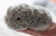
\includegraphics[keepaspectratio,width=4cm,clip]{images/previous_robots/moflin.jpg}
    \subcaption{aibo~\cite{web_moflin}}
    \label{fig:moflin}
  \end{minipage}
  \begin{minipage}[c]{0.32\linewidth}
    \centering
    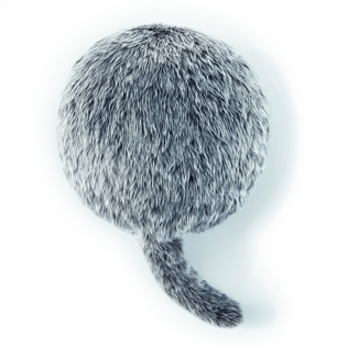
\includegraphics[keepaspectratio,width=4cm,clip]{images/previous_robots/qoobo.png}
    \subcaption{パロ~\cite{web_qoobo}}
    \label{fig:qoobo}
  \end{minipage}
  \begin{minipage}[c]{0.32\linewidth}
    \centering
    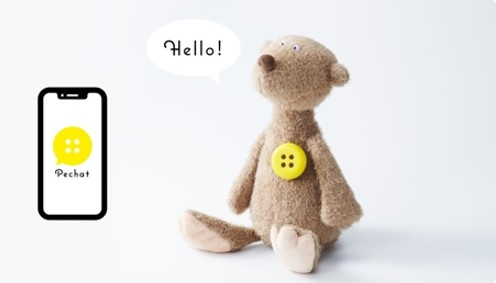
\includegraphics[keepaspectratio,width=4cm,clip]{images/previous_robots/pechat.jpg}
    \subcaption{LOVOT~\cite{web_pechat}}
    \label{fig:pechat}
  \end{minipage}
  \caption{愛玩用ロボットの例(低価格帯)}
  \label{fig:previous_robots_inexpensive}
\end{figure}


\subsection{ぬいぐるみの特徴}

そこで、人々に親しまれているぬいぐるみをロボットにすることを考える。
ぬいぐるみにはいくつかの特徴があるが、筆者の経験をもとにぬいぐるみの魅力を以下に述べる。

第一に、ぬいぐるみはその可愛らしい見た目ともふもふとした柔らかい触り心地から、落ち着きを与えてくれる。
幼い子どもがぬいぐるみとともに就寝するというのはよく見られる光景であろう。

次に、ぬいぐるみは自発的に動く存在ではなく、持ち主が触れ合いたいと考えたときだけ触れ合える。
これは、ぬいぐるみは持ち主の生活を縛らない、適度な距離感を持った愛玩対象であることを示す。
また、手入れの手間もほとんどかからないため、複数所持することは容易であり、使わない場合は長期間しまっておくことも可能である。

さらに、ぬいぐるみは人の心を投影する対象ともなりうる。
例えば図では女性が赤ちゃんにぬいぐるみを通して語りかけているが、これは女性の感情をぬいぐるみに代弁させているとも捉えられる。
つまり、ぬいぐるみとは愛玩対象であるとともに自身の代弁者ともなり、人とのコミュニケーションにおいて面と向かって伝えづらいこともぬいぐるみを通して語れるといった、コミュニケーションに彩りを持たせ、円滑に進める働きもある。

最後に、ぬいぐるみは実に多様な見た目のものが存在する。
例えば本物の動物であれば、その大きさなどの物理的制約から、実際に飼育できるものは犬や猫、小動物といったものに限られる。
一方で、ぬいぐるみは多くの種類が存在し、より個人の好みに寄り添う存在となっている。
例えば図ではアザラシやペンギン、ホッキョクグマなどを模したぬいぐるみが確認できるが、一つの店だけで50種類近くの品揃えがあることも珍しくない。
付け加えて重要なのが、これらのぬいぐるみはしばしば種々のイベントに合わせて贈られる文化が存在する点である。
子どもが誕生日に親からぬいぐるみを贈られたり、旅先の動物園や水族館、旅館等で土産に買ってもらったりすることは一般的な光景である。
そして、これらのぬいぐるみの多様性やそれにまつわる想い出は、目の前のぬいぐるみがオンリーワンの存在である印象を持ち主に与え、単なる布と綿からできた工業製品以上の愛着をもたらしうる。

このように、ぬいぐるみには様々な魅力がある一方で、それらが逆に問題となることもある。
前述のとおり、ぬいぐるみは触れ合えいたいときだけ触れ合える存在であるが、裏を返せば持ち主の働きかけがない限り決して動かないことを意味し、愛玩対象としてはやや魅力に欠ける一面がある。

本プロジェクトでは、ぬいぐるみについて、その魅力を活かしつつも、さらなる愛着を抱ける対象に発展させることを目指した。
そこで、本プロジェクトでは複数の種類のぬいぐるみを効率的にロボット化できるモジュールを開発し、持ち主の好みに寄り添ったぬいぐるみが命を吹き込まれたかのように振る舞うシステムの構築を検討した。



\section{プロジェクト概要}
本プロジェクトではぬいぐるみ専用の組み込みAIモジュールを開発し、あらゆる種類のぬいぐるみにロボティクスを適用する。
そして、幅広いぬいぐるみに効率的に知能を埋め込むためのプラットフォームの構築を目指す。

本プロジェクトでは、ぬいぐるみのロボット化に特化した組み込みAIモジュールを開発し、ぬいぐるみの骨格の規格化を目指す。そして、ぬいぐるみの毛皮と骨格の開発過程を分離することで、幅広いぬいぐるみに効率的に知能を埋め込むための土台を築き上げる。

\section{開発内容}
\subsection{骨格MohuCoreの開発}
\subsection{毛皮MohuKawaの開発}
\subsection{知能MohuAIの開発}
\subsection{ぬいぐるみロボットの完成}
\subsection{ユーザ評価}

\section{開発成果の特徴}

\section{今後の課題、展望}
本プロジェクトではシステムの簡素化及び省電力化を意図し、ロボットをESP32という比較的計算能力の低いマイクロコントローラを用いて設計した。
しかし、機械学習のスタンドアロンな実装やクラウドサービス等の連携を踏まえると、Linuxといった高機能なOSを搭載可能なシングルボードコンピュータを用いた方が発展性に富む。

本プロジェクト後半では、Raspberry Pi Zero 2Wという組み込み開発向けLinuxボードを使用し、計算能力を大幅に向上させた改良型も製作した(図)。
この改良型では、サーボモータについても電流制御等が可能で動きも滑らかな高性能なものを搭載し、ぬいぐるみロボットとしての抱き心地を改善している。

今後、ROS2といった汎用的なロボット開発フレームワークにプログラムコードを移植し、カメラや機械学習、クラウドなどとの連携が容易になる土台を整えてから、ぬいぐるみロボットのさらなる機能強化を進めたいと考えている。

展望としては、ぬいぐるみ


\section{実施計画書内容との相違点}

% \section{開発分担}

\section{成長の自己分析}
本プロジェクトではロボットの設計及び製作、ぬいぐるみの設計及び製作、ソフトウェアの作成等を一貫して行った。
その中で、ロボットの製作で何度かスクラップビルドを繰り返すなど、ハードウェアとソフトウェアともに実装能力が向上した。

しかし、一番大きな成長は、プロジェクトを進めるにあたって、本当に必要な要素は何かを常に考え、取捨選択しつつ開発を進めた点にあると考える。
ぬいぐるみロボットとはユーザの感情に訴えかける製品であり、その評価軸は必ずしも明確ではない。
今まで電子工作の技能をもっぱら自身の趣味や純粋な性能のみが重視される大学内のプロジェクトなどに捧げてきた身としては、自分の作った物についてユーザの生の声を聞き、改良に活かす本プロジェクトは非常に新鮮であり貴重な機会であった。
そして、ユーザの指摘によって自分では気づかなかったぬいぐるみロボットの問題点や新たな魅力に気づき、人との対話が製品開発には必須だと改めて気づかされることとなった。

また、未踏IT人材発掘・育成事業を通して、さまざまなPMの方々や同期のクリエータと交流が行えたことも自身の成長につながっていると考えている。
これまで大学等でものづくりについて話題を共有できる相手がほとんどおらず、孤独を感じることが多かった。
本事業では意欲のある同期のクリエータと合宿や私的な交流を通して様々な話題について議論を行った。
その内容は、各々の本事業におけるプロジェクトについてだけでなく、本事業の枠を超えた技術的・社会的問題など多岐にわたる。
本事業には所属に関係なく多様な背景や関心を持つ人材が集まっており、本事業がなければ接することのなかったであろう人々と深く討論した時間は実に有意義なものとなった。

今後も本事業を通して得られた学びやつながりを大切にし、自身のさらなる成長に活かしたいと考えている。


\section{秘匿ノウハウの指定}
本プロジェクトのソースコード等は2024年3月現在公開していない。
今後開発が進めば設計図やソースコードの公開も検討している。

\section{その他}

\section{付録}

\subsection{用語説明}
\subsubsection*{Mohutics (もふてぃくす) \label{term:mohutics}}
本プロジェクトで提案されたぬいぐるみロボットシステム及びそのシステムを採用したぬいぐるみロボットを指す。

\subsubsection*{MohuCore (もふこあ)\label{term:mohucore}}
本プロジェクトで提案されたぬいぐるみロボットシステムMohuticsにおいて、電気的・機械的要素を含むぬいぐるみロボットの骨格部分を指す。
\subsubsection*{MohuKawa (もふかわ)\label{term:mohukawa}}
本プロジェクトで提案されたぬいぐるみロボットシステムMohuticsにおいて、換装可能なぬいぐるみ部分を指す。
\subsubsection*{MohuAI (もふあい)\label{term:mohuai}}
本プロジェクトで提案されたぬいぐるみロボットシステムMohuticsにおいて、ぬいぐるみロボットに埋め込まれるソフトウェア部分を指す。

\subsubsection*{ESP32 \label{term:esp32}}
Espressif Systems社から発売されている32bitマイクロコントローラの製品群。
Wi-FiやBluetoothの搭載を特徴とし、特にESP32シリーズのマイクロコントローラを搭載したモジュールESP32-DevkitCはIoT開発を中心に広く用いられている。

\subsubsection*{IoT (Internet of Things) \label{term:iot}}
家電や車、電子機器等の様々なものがインターネットに接続され、相互に情報交換する仕組み。
本プロジェクトのぬいぐるみロボットがIoT端末として機能する場合、自宅に置いたぬいぐるみロボットをインターネット空間を経由して遠隔から操作することなどが想定される。

\subsubsection*{Linux \label{term:linux}}
コンピュータのOS(オペレーティングシステム)の一種。
オープンソースで開発されており、用途に合わせてUbuntuやDebian、Raspberry Pi OSといった様々な派生形(ディストリビューション)が存在する。


\subsubsection*{シングルボードコンピュータ \label{term:sbc}}
手のひら程度の大きさの1枚の基板にコンピュータとして必要なほぼすべての機能や要素を実装したもの。
Raspberry Pi等が知られている。

\subsubsection*{Raspberry Pi \label{term:raspi}}
Raspberry Pi財団によって開発されているARMプロセッサを搭載したシングルボードコンピュータ。
OSとしてLinuxベースのUbuntu等が使用可能な一方で、ハードウェア制御に便利な外部入出力端子を備えており、主にロボットやIoT等の組み込み用途の開発で用いられている。

\subsubsection*{ROS2 (Robot Operating System 2) \label{term:ros2}}
オープンソースのロボット用のソフトウェアプラットフォーム。
ロボットを構成するセンサやアクチュエータといった要素(ノード)同士のメッセージ通信やプログラムのパッケージ管理等を簡潔に行える。

\subsection{関連Webサイト}
\begin{description}
  \item[X: \url{https://twitter.com/mohutics}]\mbox{}\\
  プロジェクトの進捗をXのアカウントに随時掲載予定である。
  \item[GitHub: \url{https://github.com/mohutics}]\mbox{}\\
  今後ソースコードやロボットの設計図を公開する際は、このGitHubのアカウントに公開用リポジトリを掲載する予定である。
\end{description}





\bibliography{references}
\bibliographystyle{junsrt}

\end{document}
